\subsection{Baseline model architecture}
\label{sec:architecture}
The baseline architecture section describes the architecture that was used as a backbone in the REAL-TSE baseline \cite{wang2026realtse}. The architecture in this work is built from scratch, but the design is that of the baseline.
% Block diagram of the extractor as implemented. Drawn for this work.
% Provenance is stated per component in the caption, not wholesale: the diagram
% is not a redraw of any published figure -- the causal time path and the third
% input channel do not appear in one.
%
% Requires, in the preamble: \usetikzlibrary{arrows.meta,positioning,calc,backgrounds}
\begin{figure}[htbp]
\centering
\begin{tikzpicture}[
    font=\small\sffamily,
    >={Stealth[width=5pt,length=5pt]},
    block/.style={draw, fill=white, rounded corners=1.5pt, align=center, inner sep=4pt,
                  minimum height=8mm, text width=42mm},
    inblock/.style={block, text width=34mm},
    ours/.style={block, dashed, thick},
    sig/.style={font=\small, inner sep=2pt},
    note/.style={font=\scriptsize\sffamily, text=black!55},
    arr/.style={->, thick, black!75},
    skip/.style={->, thick, black!45}
  ]

  % ---------- inputs -------------------------------------------------------
  % Columns sit symmetrically about the trunk at x = 3.5 and are narrower than
  % the trunk blocks, so the upper half does not overhang it.
  \node[sig] (xin) at (0.9,0) {mixture $x$};
  \node[sig] (ein) at (6.1,0) {enrollment $e$};

  \node[inblock] (stft1) at (0.9,-1.2) {STFT\\[-1pt] \scriptsize 512 / 128, causal framing};
  \node[inblock] (stft2) at (6.1,-1.2) {STFT};

  \node[inblock] (ri)  at (0.9,-2.7) {$[\,\Re X,\ \Im X\,]$\\[-1pt] \scriptsize 2 channels};
  \node[inblock] (mag) at (6.1,-2.7) {$|X_e|$};

  \node[inblock] (tfmap) at (6.1,-4.2) {TF-Map\\[-1pt] \scriptsize spectral similarity};

  \node[ours] (cat) at (3.5,-5.7) {concatenate\\[-1pt] \scriptsize 3 input channels};

  % ---------- trunk --------------------------------------------------------
  \node[block] (split) at (3.5,-7.2)  {band split\\[-1pt] \scriptsize 32 bands over 257 bins};
  \node[block] (norm)  at (3.5,-8.7)  {per-band norm $+$ $1{\times}1$ projection\\[-1pt] \scriptsize to $N=128$};
  \node[block] (bsnet) at (3.5,-10.4) {time LSTM \emph{(causal)}\\[-1pt] $\to$ band LSTM \emph{(bidirectional)}};
  \node[block] (est)   at (3.5,-12.1) {per-band MLP\\[-1pt] \scriptsize complex mask $M$ $+$ residual $R$};
  \node[block] (apply) at (3.5,-13.6) {$\hat{S} = M \otimes X + R$};
  \node[block] (istft) at (3.5,-15.1) {inverse STFT};
  \node[sig]   (out)   at (3.5,-16.3) {estimate $\hat{s}$};

  % Six identical blocks, drawn as a stack rather than annotated with an arrow:
  % offset copies on the background layer sit behind the front block.
  \begin{pgfonlayer}{background}
    \foreach \d in {0.18,0.09}{
      \draw[draw=black!45, fill=white, rounded corners=1.5pt]
        ($(bsnet.south west)+(\d,\d)$) rectangle ($(bsnet.north east)+(\d,\d)$);
    }
  \end{pgfonlayer}
  \node[note, anchor=west] at ($(bsnet.north east)+(0.30,-0.30)$) {$\times\,6$};

  % ---------- signal flow --------------------------------------------------
  \draw[arr] (xin) -- (stft1);
  \draw[arr] (ein) -- (stft2);
  \draw[arr] (stft1) -- (ri);
  \draw[arr] (stft2) -- (mag);
  \draw[arr] (mag) -- (tfmap);
  \draw[arr] (ri.south)    -- ++(0,-0.55) -| (cat.north west);
  \draw[arr] (tfmap.south) -- ++(0,-0.55) -| (cat.north east);
  \draw[arr] (cat) -- (split);
  \draw[arr] (split) -- (norm);
  \draw[arr] (norm) -- (bsnet);
  \draw[arr] (bsnet) -- (est);
  \draw[arr] (est) -- (apply);
  \draw[arr] (apply) -- (istft);
  \draw[arr] (istft) -- (out);

  % TF-Map needs the MIXTURE magnitude as well as the enrollment's. Label sits on
  % the segment entering TF-Map, not back at the STFT it leaves.
  \draw[skip] (stft1.east) -- ++(0.75,0) |- (tfmap.west);
  \node[note] at ($(tfmap.west)+(-0.62,0.20)$) {$|X|$};

  % The complex mixture bypasses the network: the mask multiplies into it, not
  % into the network's features.
  \draw[skip] (split.east) -- ++(1.15,0) |- (apply.east);
  \node[note, align=left, anchor=west] at ($(split.east)+(1.30,-0.55)$)
        {complex\\mixture\\bands};

  % ---------- legend -------------------------------------------------------
  \node[note] at (3.5,-17.0) {\emph{dashed}: added in this work};

\end{tikzpicture}
\caption{The extractor as implemented. Band splitting and the interleaved
band-level and sequence-level modelling follow \cite{luo2023music}; the
mask-plus-residual estimator follows \cite{yu2023high}; TF-Map conditioning
follows \cite{zhang2025multi}. The causal time path and the third input channel
are this work's.}
\label{fig:baseline-architecture}
\end{figure}

\subsubsection{Band-split Recurrent Neural Network (BSRNN)}
\label{sec:bsrnn}
Luo and Yu \cite{luo2023music} propose the BSRNN model as a frequency-domain separation model that is designed for high sample rate audio, in which the input audio is transformed from its waveform representation into a time-frequency representation using the Short-Time Fourier Transform (STFT). The model then divides the input spectrum into multiple frequency bands that are modelled independently. The original use case for the BSRNN model is music source separation, but in this work, the model is adapted to allow for the extraction of a target speaker from a mixture of speech signals. The development from music source separation to the method of the target speaker extraction (TSE) approach that this work follows came from the following lineage: \textit{(i)} music source separation was adapted to personalised speech enhancement (PSE) by Yu et al. \cite{yu2023high}. The authors proposed target speaker extraction in the PSE task by appending a target speaker enrollment module that was designed to suppress any interference. PSE can be summarised as enrollment-conditioned extraction. \textit{(ii)} Zhang et al. followed this framework and proposed a new module for the enrollment conditioning module, namely the Time-Frequency Map (TF Map) \cite{zhang2025multi}.


\subsubsection{Short-time Fourier transform}
\label{sec:stft}
The model operates in the time-frequency domain rather than a waveform. To ensure the input audio is in suitable form, a short-time Fourier transform (STFT) is applied by cutting the waveform into short, overlapping frames. A window function is applied to each frame, and then a discrete Fourier transform is applied to each windowed frame. The result is a complex-valued spectrogram, a two-dimensional representation of the audio signal. On the horizontal axis is time, and on the vertical axis is frequency. The discrete Fourier transform is defined as:
\begin{equation}
X(f, t) = \sum_{n=0}^{N-1} x[tH + n]\,h[n]\,e^{-\mathrm{j}2\pi fn/N},
\label{eq:stft}
\end{equation}
 where $N$ is the window length, $H$ the hop between frames, $h[n]$ a Hann window and $\mathrm{j}$ the imaginary unit. Following Yu et al.\ \cite{yu2023high}, $N = 512$ and $H = 128$ at \SI{16}{\kHz}: a \SI{32}{\ms} window moving in \SI{8}{\ms} steps, giving 257 frequency bins. Frames are not centred on timestamps as this would imply future information which is not suitable for streaming tasks. Instead, the signal is padded with $N - H$ samples at the start of a sequence.


\subsubsection{Band plan}
\label{sec:bandplan}

The spectrogram of Section~\ref{sec:stft} has 257 outputted frequency bins, each covering an equal slice of \SI{31.25}{\Hz}. However, each band should be modelled independently. Most of the structure that distinguishes one voice from another sits at the lower frequencies: the pitch of a voice and the resonances that give a vowel its identity all fall below about \SI{4}{\kHz}, and energy falls away steadily above that. The bins near the top carry far less information and thus would be wasteful to model with the same level of detail as the bins near the bottom.  

A band plan is the decision of how to group those bins. Bins are gathered into bands and each band is then handled separately by the network: it gets its own normalisation and projection. This allows a band to be compared against itself over time rather than against the loud low-frequency bands next to it. Grouping few bins per band keeps fine detail. Secondly grouping many bins into one band summarises coarsely but costs far less. A band plan therefore decides where the model's resolution is spent. 

 The plan in this work divides the 257 bins into 32 bands: fifteen of 3 bins (about \SI{100}{\Hz}) up to \SI{1.4}{\kHz}, ten of 6 bins (about \SI{200}{\Hz}) up to \SI{3.3}{\kHz}, five of 16 bins (\SI{500}{\Hz}) up to \SI{5.8}{\kHz}, one of 64 bins (\SI{2}{\kHz}) up to \SI{7.8}{\kHz}, and a final band of the 8 remaining bins at the top of the spectrum. Figure~\ref{fig:bandplan} shows it against a real mixture in the training set. This plan follows the implementation from Zhang et al.\ \cite{zhang2025multi} for their \SI{16}{\kHz} target speaker extraction model and used by the challenge baseline built on it, but no reason is given for these particular boundaries, and no explanation is given in previous papers.

\begin{figure}[htbp]
\centering
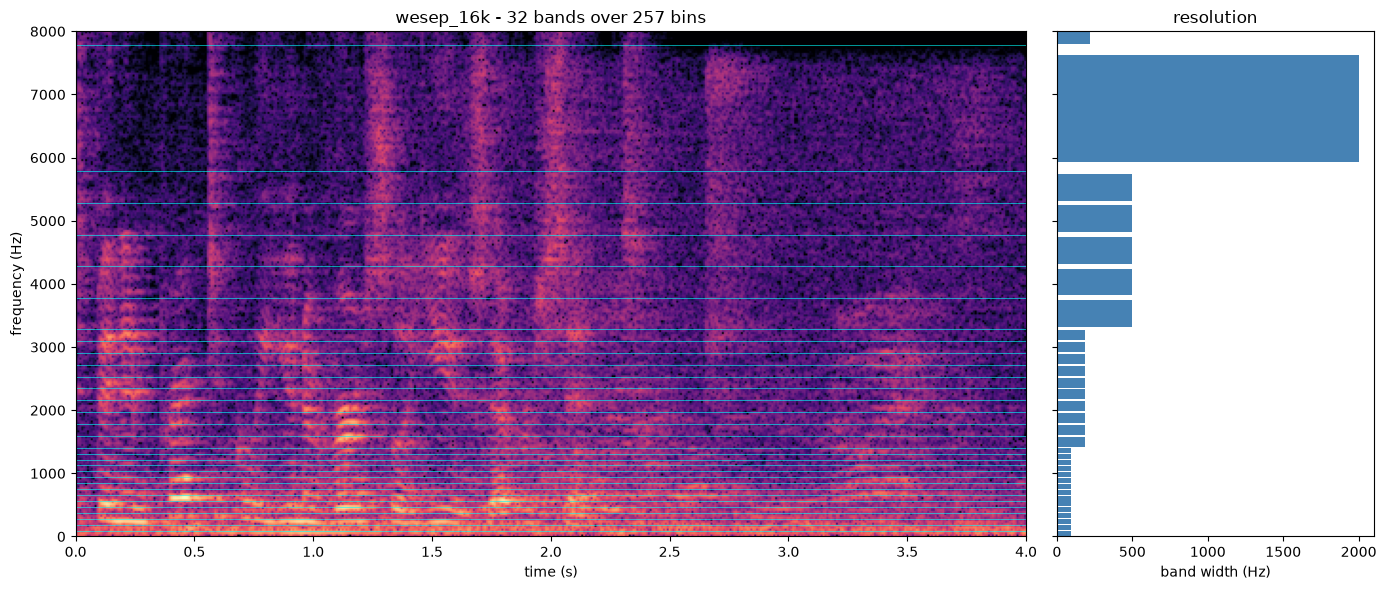
\includegraphics[width=\textwidth]{figures/bandplan-wesep.png}
\caption{The band plan used here, shown against a four-second mixture from the training set. Left: the band boundaries drawn over the spectrogram, closely spaced at the bottom where the speech structure is and widening upwards. Right: the width of each band in hertz.}
\label{fig:bandplan}
\end{figure}


\subsubsection{Per-band normalisation}
\label{sec:subbandnorm}

The bands defined by Section~\ref{sec:bandplan} are not comparable with one another. Each band typically carries different amounts of energy; therefore, if all 257 bins were scaled together, there would be a severe imbalance. The high bands would be underrepresented and thus diluted, effectively reducing the model's ability to learn the high-frequency features. Giving each band its own scaling is what prevents that. A band at \SI{6}{\kHz} is then judged against its own typical level rather than against the bands beneath it.

Following \cite{yu2023high} the approach first normalises the band, using a layer normalisation applied across the channels of that band. Secondly, because the bands must be the same size before they can be stacked together, a projection is required to map the band to a fixed width. Since there are varying sized and independent bands, each band has its own projection, which is a learnable linear layer that maps the band to a fixed width of 128 values. Every band is given the same structure but its own weights, so nothing is shared between bands and each is free to learn a representation suited to its own frequency range. The result is a stack of 32 bands, each with 128 features, which is then passed to the next module.

Normalisation is applied across the values of a band \emph{within a single frame}. Each frame is therefore normalised using only itself. This is a deliberate design choice that \emph{opposes} Yu et al.\ \cite{yu2023high}, who use batch normalisation for their online configuration. The opposition is for the following reasons: \textit{(i)} during training, the mean and variance are computed from the current batch, but during inference, these statistics are computed from the entire training set. The function that is optimised during training is therefore not the function that is deployed. \textit{(ii)} The variability of the data does not give a reliable estimate of the true distribution. The statistics of a batch therefore depend on what was drawn, and a silent crop normalised alongside loud ones is not normalised as it would be at inference. \textit{(iii)} Single frame normalisation carries no state and is unaffected by the amount of audio processed, so a four-second training chunk is normalised exactly as a stream that has been running for a minute.


\subsubsection{Residual LSTM block}
\label{sec:resrnn}

Two kinds of sequential structures are modelled: time and frequency. Time is unidirectional, but frequency is bidirectional, as all of the bands of a frame are available at the same instant and can be traversed in either direction. The block is used for both kinds of modelling, with the same structure but different parameters.

At inference time, since the model is running in a streaming fashion, the LSTM's internal state is preserved between frames and information can be carried forward indefinitely. The LSTM is therefore a natural fit for the task, and it is used in the same way for both the time and frequency sequences.

The block is made of three steps applied in order, following \cite{luo2023music}. The input is first normalised, then passed through the LSTM, and the LSTM's output is then mapped back to the input's width by a learned projection. The final addition is a residual connection and is inspired by the original ResNet \cite{he2016deep} architecture. This allows the gradient an unobstructed path back through the computation stack of all the blocks, which matters because six of these blocks are stacked in Section~\ref{sec:bsnet}. This is important as the LSTM is a deep recurrent layer, and the gradient can vanish or explode as it passes through the LSTM's internal state. The residual connection allows the gradient to bypass the LSTM entirely, which is what allows the model to train when the gradient vanishes within the LSTM. 

A single LSTM layer is given a width of 192, which is Yu et al.'s \cite{yu2023high} choice for their \SI{16}{\kHz} model. The input to the block is 128 wide, which is projected to 192 for the LSTM and then projected back to 128 for the residual addition. 

\subsubsection{Band and sequence model}
\label{sec:bsnet}

The band and sequence model is the implementation of the residual LSTM block of Section~\ref{sec:resrnn} in a stack of six blocks, using the input from Section~\ref{sec:subbandnorm}. After the per-band normalisation and projection, there are 32 bands of 128 features each.

Each of these blocks is designed to make two passes: first make a pass over the time dimension (unidirectional), and then make a pass over the frequency dimension (bidirectional). This is considered as follows:
\begin{itemize}
    \item \textbf{Time}: The recurrence goes forward only, as a backward pass would assume knowledge of future frames that have not yet arrived.
    \item \textbf{Frequency}: The recurrence goes over the bands of a frame in both directions. Frequency itself is not a causal dimension. This can be reasoned by the fact that all the bands of a frame are available simultaneously so the bidirectional recurrence does not introduce any latency. 
\end{itemize}
Pairing the two passes in a single block is the design of Luo and Yu \cite{luo2023music}, who motivate it by analogy with dual-path recurrent networks for speech separation rather than by an argument specific to bands. Stacking six such blocks follows Yu et al.\ \cite{yu2023high}, where their \SI{16}{\kHz} model uses that specific number of blocks. The effect of stacking the blocks is to allow for the accumulation of evidence over longer time spans.

\subsubsection{Estimation module}
\label{sec:estimator}

The estimation module is responsible for producing an output spectrogram that contains the estimated target speaker's speech. This is done by creating an output network per band to reconstruct the target speaker's speech from the features produced by the band and sequence model. However, there are two methods to do this: either to predict the output spectrogram directly, or to predict a mask that is applied to the mixture. The latter is the approach taken here, following Yu et al.\ \cite{yu2023high}.

Yu et al. realised that the mixture audio itself already contains the target's speech, and thus it would be more efficient to mask the mixture rather than predict the output spectrogram directly. This mask is a number for each time-frequency bin, which the mixture is multiplied by. A mask alone is not enough as multiplication can only ever scale what a bin already holds. In the cases where the interferer completely dominates a bin no multiplier recovers the target as the multiplication operation would not be able to scale the drowned out target. To solve this, the estimation module makes use of a residual spectrogram, which is predicted directly and added. Yu et al.\ \cite{yu2023high} introduce it for exactly this reason, to absorb what the mask alone produces as artefacts. It is useful to not bound this mask and is what the original implementation encouraged. The estimate for a band is then
\begin{equation}
\hat{S} = M \otimes X + R,
\label{eq:estimator}
\end{equation}
where $\otimes$ is the complex product, taken bin by bin. The $X$ that the mask multiplies is the original complex mixture and is taken as is from the band split and not from the output of the model's features. The features are used only to \emph{decide} how to mask the input. The conditioning feature of Section~\ref{sec:tfmap} therefore never enters the signal path either.

Each band has its own two-layer output network: a normalisation, then a projection to a width of 384 with a $\tanh$ activation. Finally we have two output layers reading from it, one producing the mask and one the residual. The width of 384 is the value Yu et al.\ \cite{yu2023high} specify.

The mask output layer has to output four pairs of real and imaginary parts for each frequency bin. Two of them are taken as the mask values, and the other two are passed through a sigmoid, giving a number between zero and one that each mask value is then multiplied by. This arrangement is a gated linear unit \cite{dauphin2017language}, and it is what both source papers specify for this layer \cite{luo2023music, yu2023high}.

\subsubsection{Time-frequency map}
\label{sec:tfmap}
The TF Map \cite{zhang2025multi} is the module that turns speech enhancement into target speaker extraction. It compares the mixture with the clean enrollment clip frame by frame, and gives the network a cue of what the target's spectrum should look like at each instant. Let $|X_t|$ be frame $t$ of the mixture's magnitude spectrogram and $|X_{e,j}|$ frame $j$ of the enrollment's. Every frame is first scaled to unit length, so that only the spectral \emph{shape} remains and does not keep the loudness:
  \begin{equation}
  \tilde{x}_t = \frac{|X_t|}{\big\lVert |X_t| \big\rVert},
  \qquad
  \tilde{e}_j = \frac{|X_{e,j}|}{\big\lVert |X_{e,j}| \big\rVert}.
  \label{eq:tfmap-unit}
  \end{equation}
  Each mixture frame is then compared with every enrollment frame by cosine similarity. For unit vectors this is simply the inner product. The similarities are then turned into weights that blend the enrollment frames into a template that can be referenced against the mixture frame:
  \begin{equation} 
  C_{t,j} = \big\langle \tilde{x}_t,\ \tilde{e}_j \big\rangle,
  \qquad
  A_{t,j} = \operatorname*{softmax}_{j} \big( \kappa\, C_{t,j} \big),
  \qquad
  \mu_t = \sum_{j=1}^{T_e} A_{t,j}\, \tilde{e}_j .
  \label{eq:tfmap-cos}
  \end{equation}

  Zhang et al.\ \cite{zhang2025multi} also normalise the frames and make use of cosine similarity, but they use softmax directly on the inner product rather than scaling it by a factor $\kappa = 16$. After testing it was found that since the similarities lie between $[0, 1]$, the softmax spread the weights too evenly and thus did not give a clear template. The $\kappa$ factor is therefore used to scale the similarities which sharpens the softmax to give a more distinct template. The template only describes the shape and does not indicate whether a target is speaking. As in \cite{zhang2025multi}, the energy is restored by projecting the mixture frame onto the template's direction:
  \begin{equation}
  u_t = \frac{\mu_t}{\lVert \mu_t \rVert},
  \qquad
  m_t = \big\langle\, |X_t|,\ u_t \,\big\rangle,
  \qquad
  \phi_t = m_t\, u_t ,
  \label{eq:tfmap-energy}
  \end{equation}
  where $m_t$ is a scalar per frame which describes how much of the mixture's energy lies along the target's predicted spectrum.  $\phi_t$, the template scaled by it, is the cue passed to the network. The TF Map itself has nothing to train as \eqref{eq:tfmap-unit}--\eqref{eq:tfmap-energy} contain no weights. The extra channel is the only addition as it widens the per-band projection by about \num{33000} parameters.


\subsubsection{Objective function}
\label{sec:objective}

The objective has to express two different requirements: output the target signal when it is present, otherwise, output silence. A single loss cannot serve both use cases and so the objective is split, and each crop is scored by the branch (target present versus absent) that applies to it.

Throughout, $x$ is the mixture, $s$ the target reference and $\hat{s}$ the model's output, all in the time domain over one training crop.

\paragraph{Target present.}
The first term measures how much of the output is the target and how much is everything else, following \cite{li2026cartse}. The loss needs to be invariant to the overall volume: if $\hat{s}$ has the correct shape, it should not be penalised for being loud or quiet. Therefore the first step is to find the single gain that best explains the output as a scaled copy of the target, which will be calculated as a projection, 
\begin{equation}
\alpha = \frac{\langle \hat{s},\, s \rangle}{\lVert s \rVert^2},
\qquad
s_\textup{proj} = \alpha s,
\label{eq:alpha}
\end{equation}
and then to compare the energy of that scaled target against the energy of whatever the output contains beyond it. The loss is modelled after the Scale-Invariant Signal-to-Distortion Ratio (SI-SDR). The loss is therefore,
\begin{equation}
L_\textup{pres}
  = -10 \log_{10}
    \frac{\lVert s_\textup{proj} \rVert^2}
         {\lVert \hat{s} - s_\textup{proj} \rVert^2 + \tau_\textup{pres} \lVert s_\textup{proj} \rVert^2}.
\label{eq:lpres}
\end{equation}
Lower is better. The loss is secondly in terms of decibels (dB), which is where the logarithm comes from. The $\tau_\textup{pres}$ term in the denominator is a floor. Without it a perfect output would score $-\infty$, and the gradient would keep rewarding refinement of crops that are already essentially solved. With $\tau_\textup{pres} = 10^{-3}$ the best attainable score is
\SI{-30}{dB}. This constant follows the suggestion from CARTSE \cite{li2026cartse}. The reasoning is that an output whose residual error already sits \SI{30}{dB} below the target is close enough to be treated as solved, so it would be wasteful to keep spending gradient on it. Two properties of this measure should be stated plainly, because they are what the second term exists to compensate for. The first is that everything the output contains beyond the target is collected into one denominator. Residual interfering speech, residual background noise and artefacts the model itself introduced all count identically per unit of energy, although they are not equally damaging: a fragment of the interferer left in the output can be transcribed downstream as words the target never said, whereas a diffuse artefact of the same energy usually cannot. The measure has no way to express that difference. The second is that it is an energy ratio summed over the whole crop, so it is dominated by whatever is loudest in it. Speech energy sits overwhelmingly in the low frequencies and in vowels, which means a model can score well on \eqref{eq:lpres} while reconstructing fricatives and the upper spectrum poorly. Those are the parts that carry consonant identity, and therefore much of what makes speech intelligible rather than merely present. 

\paragraph{Multi-resolution spectral term.}
Equation~\eqref{eq:lpres} is a single number computed over the whole waveform, which makes it ignore the location of errors in the spectrum. Since it cannot express \emph{where} in the spectrum the error lies, a model that reconstructs the loud low bands well and the quiet high bands poorly is barely penalised and, being scale-invariant, it does not constrain the output's absolute loudness at all. The idea is to use a loss that considers multiple resolutions of $s$ and $\hat{s}$. By considering different granularity of the spectrogram, the model is encouraged to reconstruct both the low and high frequency bands well. A spectral term allows for this following \cite{yu2023high}:
\begin{equation}
L_\textup{MR} = \frac{1}{|\mathcal{N}|} \sum_{N \in \mathcal{N}}
  \Big(
    \big\lVert\, |S_N|^{p} - |\hat{S}_N|^{p} \,\big\rVert_1
    + \big\lVert \Re S_N - \Re \hat{S}_N \big\rVert_1
    + \big\lVert \Im S_N - \Im \hat{S}_N \big\rVert_1
  \Big),
\label{eq:lmr}
\end{equation}
where $S_N$ and $\hat{S}_N$ are the spectrograms of the target and the output (Equation~\ref{eq:stft}) with window length $N$ and hop $N/4$, and each norm is averaged over its time-frequency coefficients.

Three choices inside \eqref{eq:lmr} are worth stating. The exponent $p = 0.3$ compresses magnitudes, which will highlight the quieter components relative to loud ones so that an error in a low-energy region is not diluted just because it is quiet. Without the compression the term would be dominated by the same loud low bands that already dominate \eqref{eq:lpres}. The real and imaginary terms are left uncompressed and they are what make the term sensitive to phase: a magnitude-only loss would be indifferent to the phase that the complex mask of Section~\ref{sec:estimator} is free to change. Finally the term is evaluated at several window lengths rather than one, because a single analysis window can hide errors at its own scale.

The window lengths used are \num{8}, \num{16}, \num{32} and \SI{64}{\ms}. This is with respect to the model's own \SI{32}{\ms} framing. The model builds its output by masking \SI{32}{\ms} frames and overlapping them, so the places where most errors would occur can be expected to exist at frame boundaries. The \SI{8}{\ms} and \SI{16}{\ms} windows resolve this and the \SI{64}{\ms} window catches harmonic structure that the short ones blur.

\paragraph{Target absent.}
The model should penalise any output that is not silence. This is modelled after a modified version of the absolute level loss from CARTSE \cite{li2026cartse}, where in this works the loss now contains the denominator term. 

\begin{equation}
L_\textup{abs} = 10 \log_{10}
  \frac{\lVert \hat{s} \rVert^2 + \tau_\textup{abs} \lVert x \rVert^2}
       {\lVert x \rVert^2}.
\label{eq:labs}
\end{equation}
 Including the denominator term makes the loss relative to the input, which is directly readable: \SI{0}{dB} means the output is as loud as the mixture, that is, the model did nothing; \SI{-10}{dB} means the interfering speech was suppressed by \SI{10}{dB}. The same $\tau_\textup{abs}$ floors the term at \SI{-20}{dB}, beyond which the output counts as silent. A positive value means the
model amplified the mixture, which is a direct failure. The inclusion of the denominator also allows for scale invariance, which puts the loss in the same units as the loss for the target present case.


\paragraph{Output level.}
$L_\textup{pres}$ is scale-invariant and $L_\textup{abs}$ rewards silence, leaving a gap in the training that would otherwise allow a model to simply mute its output. This gap is filled by the third term, which ensures that the model does the following: \textit{(i)} prevents the indiscriminate output of silence, and \textit{(ii)} ensures a reasonable level of output. It bounds the output level against the target's, with a dead zone of $\pm\delta$:
\begin{equation}
L_\textup{gain} = \max\!\Big(0,\ \Big|\, 20 \log_{10} \frac{\operatorname{rms}(\hat{s})}{\operatorname{rms}(s)} \Big| - \delta \Big),
\qquad \delta = \SI{3}{dB}.
\label{eq:lgain}
\end{equation}
Inside $\pm\SI{3}{dB}$ of the target's level the term is exactly zero, where $\operatorname{rms}$ is the root mean square. Its weight, $w_\textup{g} = 1.69$, is derived rather than chosen: it is the geometric midpoint of the weight at which muting stops paying (where what muting saves on \eqref{eq:labs} equals what it costs on \eqref{eq:lgain}, both weighted as in \eqref{eq:total}) and the weight where output level will outweigh the actual content extracted.


\paragraph{Combining the two branches.}
Each term is averaged over the crops it applies to, and the two averages are
weighted against one another:
\begin{equation}
L = (1 - w) \operatorname*{mean}_{\textup{target present}}
      \big[\, L_\textup{pres} + w_\textup{m} L_\textup{MR} + w_\textup{g} L_\textup{gain} \,\big]
  + w \operatorname*{mean}_{\textup{target absent}}
      \big[\, L_\textup{abs} \,\big].
\label{eq:total}
\end{equation}
 The decision to average over the crops within each branch rather than over the entire batch is deliberate. During an epoch, a random crop can draw a trial whose label says both target and interferer are present, but the crop itself may contain silence (occurs in \SI{5.8}{\percent} of cases). The model should therefore be rewarded for silence where the loss should not be diluted by the presence of other crops in the batch. Therefore the branch a crop belongs to is decided from the audio of the cropped target itself, not from the trial's label.

\paragraph{Weights.} 

The weight $w$ on the silent branch is derived rather than chosen. Silent crops make up a measured \num{0.297} of the training crops and, following \cite{li2026cartse}, each silent crop is counted twice ($\eta = 2$). The present branch then carries $1 - p = 0.703$ and the absent branch $\eta p = 0.594$, and normalising the two to sum to one gives
  \begin{equation*}
  w = \frac{\eta p}{(1 - p) + \eta p} = \frac{0.594}{1.297} = 0.458 .
  \end{equation*}



The weight $w_\textup{m}$ on the spectral term is derived from the target present and absent losses. The reason for this term is that equations~\eqref{eq:lpres} and \eqref{eq:lmr} are in different units. $L_\textup{pres}$ is in units with respect to a ratio in decibels, and $L_\textup{MR}$ is the mean absolute difference between compressed magnitudes. Therefore the weighting term $w_\textup{m}$ will reconcile the two terms to be on the same scale.
This is done by evaluating on the output that does nothing at all, $\hat{s} = x$, over 300 training crops which will simulate the scenario for the average losses for an untrained model. The median values for $L_\textup{pres}$ and $L_\textup{MR}$ are \num{-5.91} and \num{0.184} respectively. The aim is for the spectral term (Multi-Resolution) to be roughly \SI{30}{\percent} of the present branch at the start of training. The calculation then becomes  
 $$w_\textup{m} = \frac{0.3 \times |L_\textup{pres}|}{L_\textup{MR}} =  \frac{0.3 \times 5.9088}{0.1842} = 9.62$$


